\chapter{METODOLOGI}
\label{chap:metodologi}

% Ubah bagian-bagian berikut dengan isi dari desain dan implementasi

\usetikzlibrary{positioning, fit, calc}   
\tikzset{block/.style={draw, thick, text width=2.5cm ,minimum height=1.3cm, align=center},   
	line/.style={-latex}     
}   

Penelitian ini dilaksanakan sesuai dengan desain sistem serta implementasinya. Desain sistem meliputi konsep serta langkah-langkah pembuatan dan perancangan infrastruktur yang digambarkan dalam bentuk blok-blok alur pengerjaan. Bagian implementasi berisikan pelaksanaan teknis untuk setiap blok pada desain sistem


\section{Peralatan}
\label{sec:peralatan}

Peralatan yang digunakan pada Tugas Akhir ini antara lain adalah Free Music Archive (FMA) Dataset, Google Colab, Anaconda Navigator, Visual Studio Code, Laptop, dan Desktop PC.

\subsection{Free Music Archive}
\label{subsec:fma}
Free Music Archive (FMA) merupakan sebuah dataset open-source yang biasa digunakan untuk keperluan Music Information Retrieval (MIR), seperti pengolahan data audio musik beserta fitur-fiturnya. Dataset ini berisikan sejumlah file sebesar 917 GB yang berisikan 106.754 trek musik dari 16.341 artis dan 14.854 album dengan metadatanya seperti ID, title, artist, genres, tags, dan play counts. Pada dataset ini terdapat total 161 genre (termasuk subgenre) yang tersusun secara hierarkis\citep{DBLP:journals/corr/BenziDVB16}.

\subsection{Anaconda Navigator}
\label{subsec:anacondanav}
Anaconda Navigator merupakan sebuah Graphical User Interface (GUI) untuk mendistribusikan Python dan R untuk segala keperluan komputasi ilmiah. Pada penelitian ini, Anaconda Navigator digunakan untuk men-deploy VS Code, serta instalasi segala package yang diperlukan.

\subsection{Visual Studio Code}
\label{subsec:vscode}
Visual Studio Code (VS Code) merupakan sebuah editor source code yang dikembangkan oleh Microsoft dan dapat digunakan untuk sistem operasi Windows, Linux, dan MacOS. Pada penelitian ini VS Code, disambungkan dengan Anaconda, digunakan untuk melakukan preprocessing serta training dataset.

\subsection{Desktop PC}
\label{subsec:desktop}
Desktop PC digunakan sebagai device untuk menjalankan Visual Studio Code dan penulisan buku. Berikut spesifikasi Desktop PC sesuai yang tertera pada Tabel 3.1.

\begin{table}[h]
	\centering
	
	\caption{Spesifikasi Desktop PC}
	\begin{adjustbox}{width=0.7\columnwidth, center}
	\begin{tabular}{|c|c|}
		\hline
		\textbf{Processor}        & Intel(R) Core(TM) i7-4790 CPU @ 3.60GHz \\ \hline
		\textbf{RAM}              & 16 GB DDR3                                \\ \hline
		\textbf{Storage}          & SSD 512 GB + HDD 1 TB                         \\ \hline
		\textbf{Graphics Card}    & AMD Radeon RX 5600 XT 6GB        \\ \hline
		\textbf{Operating System} & Windows 10 Home                           \\ \hline
	\end{tabular}
	\end{adjustbox}
	\label{fig:desktoptable}
\end{table}

\subsection{Laptop}
\label{subsec:laptop}

	Laptop digunakan untuk berbagai macam hal. Antara lain adalah sebagai device untuk menjalankan Visual Studio Code, melakukan training dataset, dan penulisan buku. Berikut spesifikasi laptop sesuai yang tertera pada Tabel 3.2.
	
	\begin{table}[h]
		\centering
		
		\caption{Spesifikasi Laptop}
		\begin{adjustbox}{width=0.7\columnwidth, center}
		\begin{tabular}{|c|c|}
			\hline
			\textbf{Processor}        & Intel(R) Core(TM) i5-10200H CPU @ 2.40GHz \\ \hline
			\textbf{RAM}              & 16 GB DDR4                                \\ \hline
			\textbf{Storage}          & SSD 512 GB + 1 TB                         \\ \hline
			\textbf{Graphics Card}    & Nvidia GeForce RTX 3060 6GB Laptop        \\ \hline
			\textbf{Operating System} & Windows 10 Home                           \\ \hline
		\end{tabular}
	\end{adjustbox}
		\label{fig:laptoptable}
	\end{table}

\section{Desain Sistem}
\label{sec:desainsistem}

Tugas Akhir ini mengimplementasikan Deep Learning untuk mengklasifikasikan subgenre dari suatu input potongan trek musik 30 detik yang berasal dari genre yang berbeda-beda menggunakan algoritma Convolutional Neural Network (CNN).

\begin{figure}[H]
	\centering
	
	% Ubah dengan nama file gambar dan ukuran yang akan digunakan
	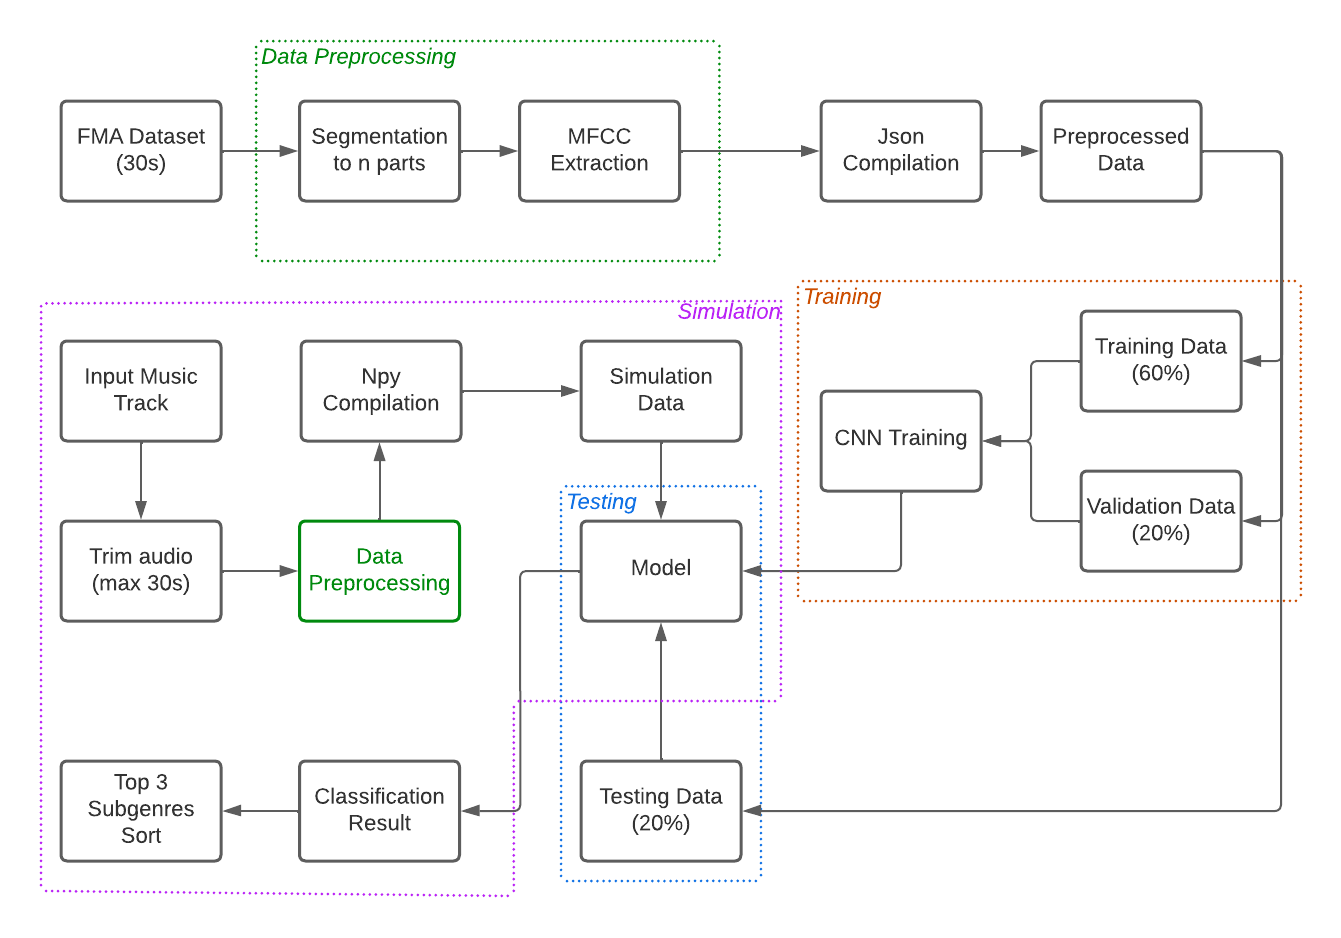
\includegraphics[width=1\textwidth]{gambar/desain sistem3}
	
	% Ubah dengan keterangan gambar yang diinginkan
	\caption{Desain Sistem}
	\label{fig:desainsistem}
\end{figure}

Tahapan sistem klasifikasi subgenre musik sesuai pada Gambar 3.1:

\begin{enumerate}
	\item Pengumpulan Data
	
	Dataset yang digunakan adalah \emph{Free Music Archive} (FMA) \citep{DBLP:journals/corr/BenziDVB16} yang berisikan potongan-potongan musik dengan durasi 30 detik yang sudah dilabeli subgenrenya.
	\item Preprocessing Data
	
	Tahap ini meliputi pemotongan input trek menjadi beberapa segmen serta ekstraksi MFCC yang kemudian dikompilasikan di sebuah file json.
	\item Training
	
	Training dataset dilakukan pada model CNN yang telah dirancang.
	
	\item Testing
	
	Mengevaluasi model yang telah dilakukan training menggunakan testing data yang kemudian dihitung akurasinya.
	
	\item Simulasi
	
	Setelah mendapatkan model yang optimal, sistem dapat digunakan untuk mengklasifikasikan suatu input musik ke dalam 3 subgenre yang paling masuk akal.
	
\end{enumerate}

\section{Pengumpulan Dataset}
\label{sec:pengumpulan dataset}

Dataset yang digunakan merupakan kumpulan musik dari 3 Genre, yaitu Rock, Folk, dan Electronic. Lalu, diambil masing-masing 3 Subgenre dengan jumlah trek sebanyak 200 tiap subgenrenya sehingga mencapai total 2700 trek. Kumpulan musik ini berupa file mp3 dari potongan 30 detik lagu yang disediakan oleh Free Music Archive(FMA) \citep{DBLP:journals/corr/BenziDVB16}. FMA ini sendiri merupakan sebuah website yang berisikan kumpulan musik-musik royalty-free. Berikut tabel dataset yang digunakan untuk training ini tertera pada Tabel 3.3.

\begin{table}[h]
	\centering
	
	\caption{Dataset yang digunakan}
	
	\begin{tabular}{|c|c|c|}
		\hline
		\textbf{Genre}              & \textbf{Subgenre} & \textbf{Jumlah} \\ \hline
		\multirow{3}{*}{Rock}       & Loud Rock         & 200             \\ \cline{2-3} 
		& Noise Rock        & 200             \\ \cline{2-3} 
		& Post Rock         & 200             \\ \hline
		\multirow{3}{*}{Folk}       & Freak Folk        & 200             \\ \cline{2-3} 
		& Free Folk         & 200             \\ \cline{2-3} 
		& Psych Folk        & 200             \\ \hline
		\multirow{3}{*}{Electronic} & Chiptune          & 200             \\ \cline{2-3} 
		& Glitch            & 200             \\ \cline{2-3} 
		& House             & 200             \\ \hline
	\end{tabular}
	
	\label{fig:dataset}
\end{table}

\section{Preprocessing Data}
\label{sec:preprocessing}

Sebelum dataset kumpulan musik diolah, perlu untuk dilakukan ekstraksi fitur yang dibutuhkan terlebih dahulu. Fitur yang digunakan pada Tugas Akhir ini adalah Mel-frequency cepstral coefficients (MFCC). Sebelum ekstraksi, dilakukan segmentasi file audio menjadi 10 segmen. Dengan ini, maka didapat potongan 3 detik sebanyak 10 buah per trek musik 30 detik. Hal ini dilakukan untuk memperbanyak jumlah data untuk training karena pada \emph{deep learning} pada umumnya diperlukan jumlah dataset yang relatif lebih banyak dibandingkan dengan \emph{machine learning} klasik. 

\begin{table}[H]
	
	\centering
	
	\caption{Parameter MFCC}
	
	\begin{tabular}{|l|l|}
		\hline
		\textbf{Parameter} & \textbf{Keterangan} \\ \hline
		Sample Rate        & 22050               \\ \hline
		N FFT              & 2048                \\ \hline
		Hop Length         & 512                 \\ \hline
		N MFCC             & 13                  \\ \hline
	\end{tabular}

	\label{fig:mfccparameter}
\end{table}

Setelah segmentasi, dilakukan ekstraksi MFCC dengan parameter seperti yang tertera pada Tabel 3.3. Berikut Gambar 3.2 adalah hasil contoh ekstraksi trek musik 30 detik menjadi 10 segmen MFCC.

\begin{figure}[H]
	\centering
	
	% Ubah dengan nama file gambar dan ukuran yang akan digunakan
	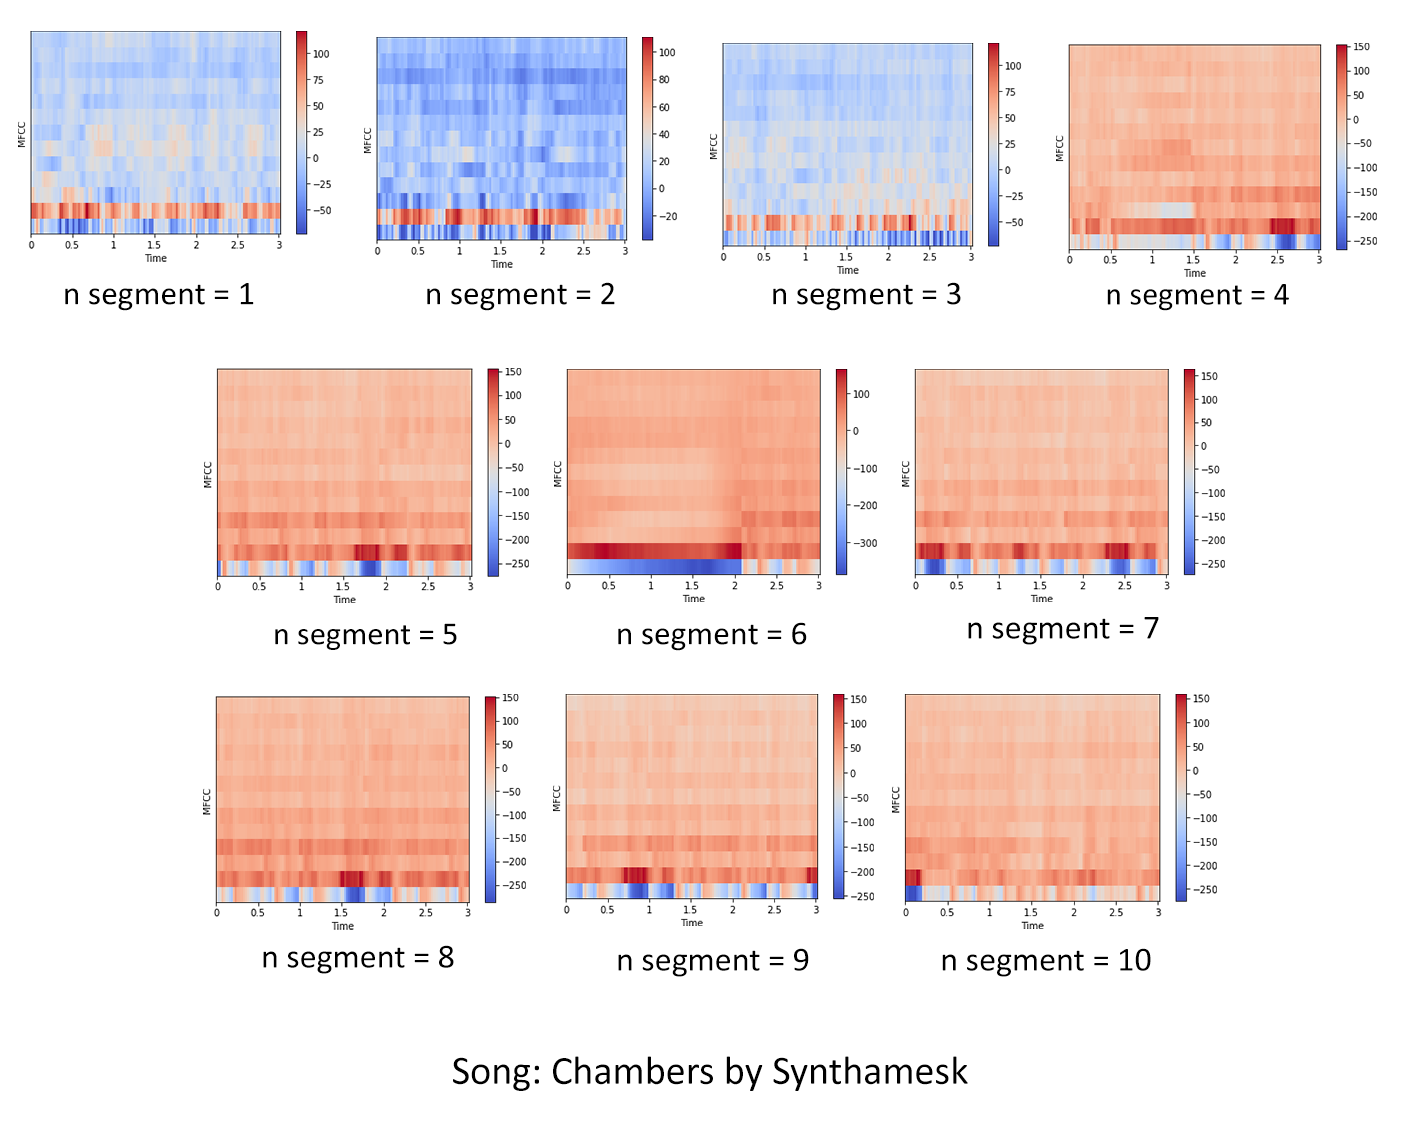
\includegraphics[width=\textwidth]{gambar/mfcc segments1}
	
	% Ubah dengan keterangan gambar yang diinginkan
	\caption{Plotting MFCC 10 Segmen}
	\label{fig:mfccsegmen}
\end{figure}

Ekstraksi dilakukan dengan menggunakan library dari python yang bernama LibROSA. Hasil ekstraksi MFCC tiap segmennya dilakukan transpose, kemudian dikompilasikan ke dalam sebuah file json. Pada file tersebut juga diberikan labeling untuk tiap subgenre (total 9 label) dan mapping untuk masing-masing label (0-8).

\section{Training}
\label{sec:training}

Setelah didapatkan hasil pemrosesan dataset serta pelabelannya, dilakukan training dataset agar komputer dapat mempelajari karakteristik dari masing-masing subgenre menggunakan fitur MFCC-nya. Dataset dibagi menjadi 3, yaitu Training Data (60\%), Validation Data (20\%), dan Test Data (20\%). Proses training dilakukan menggunakan framework Convolutional Neural Network (CNN). Layer disusun seperti yang tertera pada Tabel 3.5.

\begin{table}[h]
	\centering
	
	\caption{Susunan Layer CNN}
	
	\begin{tabular}{|l|l|l|}
		\hline
		\textbf{Layer (type)}                        & \textbf{Output Shape} & \textbf{Param \#} \\ \hline
		conv2d\_6 (Conv2D)                           & (None, 128, 11, 32)   & 320               \\ \hline
		max\_pooling2d\_6 (MaxPooling2D)             & (None, 64, 6, 32)     & 0                 \\ \hline
		batch\_normalization\_6 (BatchNormalization) & (None, 64, 6, 32)     & 128               \\ \hline
		activation\_6 (Activation)                   & (None, 64, 6, 32)     & 0                 \\ \hline
		dropout\_6 (Dropout)                         & (None, 64, 6, 32)     & 0                 \\ \hline
		conv2d\_7 (Conv2D)                           & (None, 62, 4, 64)     & 18496             \\ \hline
		max\_pooling2d\_7 (MaxPooling2D)             & (None, 31, 2, 64)     & 0                 \\ \hline
		batch\_normalization\_7 (BatchNormalization) & (None, 31, 2, 64)     & 256               \\ \hline
		activation\_7 (Activation)                   & (None, 31, 2, 64)     & 0                 \\ \hline
		dropout\_7 (Dropout)                         & (None, 31, 2, 64)     & 0                 \\ \hline
		conv2d\_8 (Conv2D)                           & (None, 30, 1, 32)     & 8224              \\ \hline
		max\_pooling2d\_8 (MaxPooling2D)             & (None, 15, 1, 32)     & 0                 \\ \hline
		batch\_normalization\_8 (BatchNormalization) & (None, 15, 1, 32)     & 128               \\ \hline
		activation\_8 (Activation)                   & (None, 15, 1, 32)     & 0                 \\ \hline
		flatten\_2 (Flatten)                         & (None, 480)           & 0                 \\ \hline
		dense\_4 (Dense)                             & (None, 64)            & 30784             \\ \hline
		dropout\_8 (Dropout)                         & (None, 64)            & 0                 \\ \hline
		dense\_5 (Dense)                             & (None, 9)             & 585               \\ \hline
	\end{tabular}

	\label{fig:layercnn}
\end{table}

Konfigurasi yang digunakan pada model dapat dilihat seusai seperti yang tertera pada Tabel 3.6.

\begin{table}[h]
	
	\centering
	
	\caption{Konfigurasi Model}
	
	\begin{tabular}{|l|l|}
		\hline
		\textbf{Jenis Konfigurasi} & \textbf{Keterangan} \\ \hline
		Classes                    & 9                   \\ \hline
		Batch                      & 8/16/32                 \\ \hline
		Epoch                      & 80/100                  \\ \hline
	\end{tabular}

	\label{fig:konfigurasimodel}
\end{table}

Classes merupakan jumlah label subgenre yang ingin diklasifikasikan. Batch size menentukan jumlah segmen MFCC yang diproses tiap Epoch-nya. Pada penelitian ini digunakan 3 Batch Size serta 2 Epoch yang berbeda untuk pengujian. 

\section{Testing}
\label{sec:testing}

Pada tahap testing, dilakukan perhitungan serta plotting confusion matrix untuk dapat melihat performa model untuk mengklasifikasikan masing-masing subgenre. Selain itu, dapat juga diketahui similaritas dari masing-masing subgenre serta hubungan antara satu dengan yang lainnya. Selanjutnya, dilakukan percobaan dengan input trek musik dengan berbagai macam durasi (maksimal 30 detik) dan melihat prediksi yang dilakukan oleh sistem dengan cara menampilkan 3 subgenre dengan probabilitas tertinggi.

\section{Rencana Pengujian dan Simulasi}
\label{sec:rencanapengujian}

Pada tahap ini dilakukan beberapa pengujian untuk mengetes performa dari implementasi sistem. Tahap pengujain dibagi menjadi beberapa bagian, yaitu:

\begin{enumerate}
	\item Pengujian pengaruh batch size dan epoch terhadap model
	\begin{enumerate}
		\item Batch size = 8; Epoch = 80
		\item Batch size = 8; Epoch = 100
		\item Batch size = 16; Epoch = 80
		\item Batch size = 16; Epoch = 100
		\item Batch size = 32; Epoch = 80
		\item Batch size = 32; Epoch = 100
	\end{enumerate}
	
	\item Pengujian pengaruh durasi input audio terhadap hasil klasifikasi
	\begin{enumerate}
		\item 30 detik
		\item 15 detik
		\item 9 detik
		\item 3 detik
	\end{enumerate}
	
\end{enumerate}